\documentclass{ceurart}

\usepackage{caption}
\usepackage{subcaption}
\usepackage{listings}
\usepackage{xspace}
\usepackage{xcolor}
\usepackage{relsize}
\usepackage{tikz}
\usepackage{tabularx}
\usepackage{multirow}
\usepackage{sourcecodepro}
\usepackage{csquotes}
\usepackage{bm}

\usetikzlibrary{arrows.meta}
\usetikzlibrary{positioning}

\lstset{breaklines=true}

\newcommand{\todo}[1]{\textcolor{blue}{#1}}
\newcommand{\todocite}{\todo{[CITE]}\xspace}

\newcommand{\Ni}{(1)~}
\newcommand{\Nii}{(2)~}
\newcommand{\Niii}{(3)~}
\newcommand{\Niv}{(4)~}
\newcommand{\Nv}{(5)~}
\newcommand{\Na}{(a)~}
\newcommand{\Nb}{(b)~}
\newcommand{\Nc}{(c)~}
\newcommand{\Nd}{(d)~}
\newcommand{\Ne}{(e)~}

\newcommand{\textttsmall}[1]{\texttt{\smaller #1}}
\newcommand{\query}[1]{\textttsmall{#1}}
\newcommand{\Bert}{\textsc{Bert}\xspace}
\newcommand{\iraxioms}{\textttsmall{ir\_axioms}\xspace}
\newcommand{\nDCG}[1]{nDCG\def\tempndcg{#1}\ifx\tempndcg\empty\else{@}\tempndcg\fi}
\newcommand{\map}{MAP}
\newcommand{\KwikSort}{\textsc{KwikSort}\xspace}
\newcommand{\redtext}[1]{{\color{red} (#1)}}

\begin{document}

\copyrightyear{2022}
\copyrightclause{%
  Copyright for this paper by its authors.
	Use permitted under Creative Commons License Attribution~4.0
	International~(CC~BY~4.0).%
}
\conference{%
  CLEF~2022: 
  Conference and Labs of the Evaluation Forum, 
	September~5--8,~2022,
  Bologna, Italy%
}

\title{%
  Grimjack at \texorpdfstring{Touché~2022}{Touché 2022}:\texorpdfstring{\\}{ }
  Axiomatic Reranking and Query Reformulation%
}
\title[mode=sub]{%
  Notebook for the Touché Lab on Argument Retrieval at CLEF\ 2022%
}

\author{Jan Heinrich Reimer}[
  orcid=0000-0003-1992-8696,
  email=jan.reimer@student.uni-halle.de,
  url=https://heinrich.reimer.family,
]
\author{Johannes Huck}[
  email=johannes.huck@student.uni-halle.de,
  url=https://github.com/johannes-huck,
]
\author{Alexander Bondarenko}[
  orcid=0000-0002-1678-0094,
  email=alexander.bondarenko@informatik.uni-halle.de,
  url=https://alexanderbondarenko.com/,
]

\address{%
  Martin-Luther-Universität Halle-Wittenberg,
  06099~Halle~(Saale), Germany
}

\begin{abstract}
%  We, Team Grimjack, present our approach for answering comparative questions, submitted in five runs to the Touché Lab on Argument Retrieval.
%  Our approach follows two objectives: ranking argumentative and high-quality documents first, and exposing arguments of different stances towards the compared objects fairly in high ranking positions.
%  We therefore propose a multi-stage retrieval pipeline with query reformulation and combination, baseline retrieval, quality and stance tagging, and different task-specific re-ranking steps.
%  First, we re-rank axiomatically based on argumentative retrieval axioms.
%  Second, we re-rank to ensure fair exposure across argument stances.
%  In all retrieval steps, we use the T0 language model to evaluate whether zero-shot language models can successfully answer comparative questions.
In this paper, we present the Team's Grimjack retrieval approaches for the Touch{\'e} shared task on Argument Retrieval for Comparative Questions. In total, we submitted five runs that pursue the two main objectives: favoring argumentative and high argument quality documents in the final ranking and addressing a retrieval ``fairness'' by ensuring an even ratio of pro and con arguments at top ranks.
%proposed alternative that might be enough for now. Once we have official evaluation results, we can add a sentence or two on that.
\end{abstract}

\begin{keywords}
  Axiomatic Re-ranking \sep
  Query Reformulation \sep
  T0 \sep
  Argument Quality \sep
  Argument Stance \sep
  CEUR-WS
\end{keywords}


\maketitle

\section{Introduction}\label{intro}

Argument retrieval is a specific task that not only considers topical relevance of retrieved documents to given queries (usually of controversial, argumentative or opinion nature) but also accounts for argument specific features like argument quality and stance~\cite{BondarenkoFBGAPBSWPH2020, BondarenkoGFBAPBSWPH2021}.  
Furthermore, it has been shown that current search engines might return biased results~\cite{ShahB2022} and argument retrieval systems return ``unfairelly'' distributed pro / con arguments~\cite{CherumanalSSC2021}.
We especially emphasize the importance of retrieving diverse results for comparative questions (e.g., ``Train or plane? Which is the better choice?'') that provide different point of views to mitigate biasing users' decisions towards one or the other comparison option.

Our Team Grimjack participated in the Touch{\'e} shared task on Argument Retrieval for Comparative Questions which goals are: \Ni To retrieve relevant and high quality argumentative passages from a collection of 868\,655~text passages to a set of 50~search topics and \Nii to classify the stance of the retrieved passages towards the comparison objects in search topics~\cite{BondarenkoFKSGBPBSWPH2022}.
As part of our participation in the task, we have developed a flexible retrieval pipeline in Python based on Pyserini~\cite{LinMLYPN2021} as an easily configurable command line application.
In the first step, our approach uses query (comparative questions from topics' titles) reformulation and expansion by important terms from topics' descriptions and narratives. Then the top~100 initially retrieved passages using query likelihood with Dirichlet smoothing~\cite{ZhaiL2001} are axiomatically re-ranked based on the number and position of premises, claims, and comparative objects (identified with TARGER~\cite{ChernodubOHBHBP2019}) and argument quality predictions by the IBM Debater API~\cite{ToledoGCFVLJAS2019} and T0++~\cite{SanhWRBSACSLRDBXTSSKCNDCJWMSYPBWNRSSFFTBGBWR2021}.
Finally, the pro and con argumentative passages towards the comparative objects are balanced in the final ranking by alternating documents of different stance (cf.\ Section~\ref{approach} for more details on the approach and submitted runs).

Additionally, we manually labeled the \todo{relevance} of \todo{XX} documents for three topics returned by our system (before the official results are made available by the organizers). Our manual assessment shows the potential of expanding queries with synonyms and contextual information for improving the effectiveness of our argument retrieval approach~(cf.\ Section~\ref{evaluation}).

%% The last statement could fit in the CR version depending on the final evaluation: good or bad
%Different configurations for our submitted runs should pose examples to discuss current doubts about the usefulness of large zero-shot language models like T0++~\cite{SanhWRBSACSLRDBXTSSKCNDCJWMSYPBWNRSSFFTBGBWR2021} in the field of argumentative information retrieval~\cite{ShahB2022}.

\section{Related Work}

Personal decision making often starts with formulating comparative questions like ``Should I major in philosophy or psychology?''~\cite{BondarenkoFBGAPBSWPH2020,BondarenkoGFBAPBSWPH2021,BondarenkoFKSGBPBSWPH2022}. Short direct answers (potentially biased)~\cite{PotthastHS2020} to such questions might be insufficient; instead, such questions require diverse opinions to provide a sufficient, balanced, and argumentative overview~\cite{BondarenkoFBGAPBSWPH2020}.
The Touch{\'e} shared task on Argument Retrieval for Comparative Questions was proposed to evaluate retrieval approaches on a large corpus with respect to relevance and rhetorical quality of potential answers to comparative questions that also may represent different standpoints~\cite{BondarenkoFKSGBPBSWPH2022,BondarenkoADHBH2022}.

The most effective approaches at previous Touch{\'e} editions~\cite{BondarenkoFBGAPBSWPH2020,BondarenkoGFBAPBSWPH2021} successfully used query expansion with synonyms and antonyms~\cite{AbyeST2020}, identified premises and claims in retrieved documents~\cite{Huck2020, ShirshakovaW2021}, estimated argument quality~\cite{AbyeST2020}, and re-ranked initially retrieved documents based on argument quality and document ``comparativeness'', e.g., a ratio of comparative adjectives~\cite{ChekalinaP2021}. Inspired by the participant approaches from the previous Touch{\'e} editions, we also include the components of argument mining and argument quality estimation in our retrieval pipeline, however, using different methods.
We rely on a large language model~T0 trained in multitask setting that showed to achieve state-of-the-art results for various Natural Language Processing tasks in zero-shot settings~\cite{SanhWRBSACSLRDBXTSSKCNDCJWMSYPBWNRSSFFTBGBWR2021}. The largest pretrained T0 variant, T0++, was trained on 62~datasets with 12~task-specific prompts covering such tasks as question answering, sentiment analysis, summarization, etc. By using T0++, we aim for answering a question whether the abilities of large language models are sufficient for the new task of argument retrieval.

Our second idea of axiomatic re-ranking comes from axiomatic thinking in information retrieval, where axioms formally describe constraints that good retrieval model should fulfil, e.g., documents with more query term occurrences should be ranked higher~\citet{FangTZ2004}. It has already been shown that combining multiple axioms for re-ranking results of arbitrary retrieval models can improve final overall retrieval effectiveness~\cite{HagenVGS2016}. Complementing existing retrieval axioms, \citet{BondarenkoHVSPB2018} introduced argumentativeness axioms based on claims and premises in documents identified with TARGER~\cite{ChernodubOHBHBP2019}.

\section{Approach}\label{approach}

\begin{figure}
	\centering
    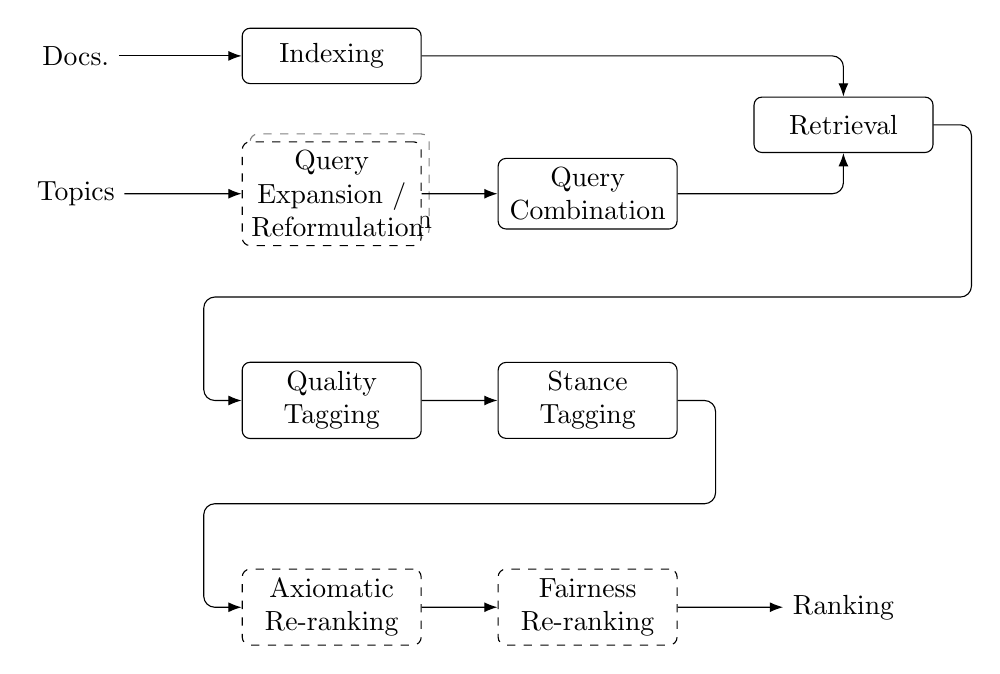
\begin{tikzpicture}[
        xscale=3.25,
        yscale=-1.75,
        block/.style={
            rectangle,
            draw,
            fill=white,
            text centered,
            rounded corners=1mm,
            text width=5.8em,
            minimum height=2em
        },
        line/.style={
            draw,
            -Latex,
            rounded corners
        },
        ]

        \node (documents) at (0,0) {Docs.};
        \node [block] (index) at (1,0) {Indexing};
        \node (topics) at (0,1) {Topics};
        \node [block,dashed,draw opacity=0.5,xshift=1mm,yshift=1mm] at (1,1) {Query Expansion / \\ Reformulation};
        \node [block,dashed] (query-expansion-reformulation) at (1,1) {Query Expansion / \\ Reformulation};
        \node [block] (query-combining) at (2,1) {Query Combination};
        \node [block] (retrieval) at (3,0.5) {Retrieval};
        \node [block] (quality-tagging) at (1,2.5) {Quality Tagging};
        \node [block] (stance-tagging) at (2,2.5) {Stance Tagging};
        \node [block,dashed] (axiomatic-reranking) at (1,4) {Axiomatic Re-ranking};
        \node [block,dashed] (fairness-reranking) at (2,4) {Fairness Re-ranking};
        \node (ranking) at (3,4) {Ranking};
ranking
        \path [line] (documents) -- (index);
        \path [line] (topics) -- (query-expansion-reformulation);
        \path [line] (query-expansion-reformulation) -- (query-combining);
        \path [line] (index) -| (retrieval);
        \path [line] (query-combining) -| (retrieval);
        \path [line] (retrieval) -| (3.5,1.5) |- (2,1.75) -| (0.5,2) |- (quality-tagging);
        \path [line] (quality-tagging) -- (stance-tagging);
        \path [line] (stance-tagging) -| (2.5,3) |- (2,3.25) -| (0.5,3.5) |- (axiomatic-reranking);
        \path [line] (axiomatic-reranking) -- (fairness-reranking);
        \path [line] (fairness-reranking) -- (ranking);
    \end{tikzpicture}\\[0.75em]
	\caption{Architecture overview for the retrieval pipeline used to produce our runs. Dashed boxes indicate optional steps, that are not used in all runs.}
    \label{figure-pipeline}
\end{figure}


We design the architecture of our argumentative retrieval system as a pipeline of multiple steps that subsequently (re-)rank, annotate, or modify the documents or queries given as inputs. This pipeline is shown in Figure~\ref{figure-pipeline}.
We identify four core steps as most important to our approach:
\Ni query expansion, reformulation, and combination,
\Nii first-stage retrieval,
\Niii argument quality and stance tagging,
and \Niv axiomatic reranking and fairness reranking.

Additionally, we add an evaluation component that is not shown in Figure~\ref{figure-pipeline} because it is not needed to retrieve results from our system.
With this evaluation component we can evaluate our system on topics of previous editions~(i.e.,~2021 and~2020) of the Touché Lab on Argument Retrieval~(c.f.~Section~\ref{transfer-relevance-judgements}).

\subsection{Query Expansion, Reformulation, and Combination}
\label{reformulation}

In order to increase recall of our first-stage ranker and to include results for very similar yet differently named objects, we first expand and reformulate the original search query.
Our approaches use two different strategies: \Ni we replace the comparative objects with their synonyms and \Nii we generate additional, new queries using the additional description and narrative information provided by the shared task organizers~\cite{BondarenkoFKSGBPBSWPH2022}.
Expanding the original query with synonyms of comparative objects is motivated by the fact that documents often contain more specific comparisons~(e.g., Ubuntu vs Windows) instead of more broad comparisons~(e.g., Linux vs Windows).
Yet, specific examples of a more general class of objects are useful to answer comparative questions about their object class.
We might therefore find relevant documents that would otherwise not match any original query term.
It is however important to note that increasing recall can result in an decrease in precision which is undesirable in the precision-oriented setting of the shared task.
However, we later apply re-ranking steps that improve precision by moving irrelevent documents further down the ranking~(c.f.~Section~\ref{reranking}).

\paragraph{Query Expansion with Synonyms}

We use two different strategies to find synonyms: \Ni word embeddings and \Nii a zero-shot language model.
In our first strategy, we use fastText word embeddings~\cite{BojanowskiGJM2017} to find words with the highest cosine similarity to the given comparative objects in the embedding space.
We manually examine synonyms from fastText embeddings using different domains~(i.e., Wikipedia and Twitter) and find that fastText embeddings trained on the Twitter corpus result in the best synonyms.

Our second strategy to obtain synonyms is based on the T0++~zero-shot language model~\cite{SanhWRBSACSLRDBXTSSKCNDCJWMSYPBWNRSSFFTBGBWR2021}.
We ask the model to generate an answer to the following task: \query{What are synonyms of the word~<token>?} where \query{<token>}~is one of the two comparative objects.
From the text returned by the language model, we then parse synonyms by splitting at commas and remove duplicate synonyms.
With the synonyms returned by either strategy, we replace the comparative objects to form new queries. All alternative queries and the original query are then combined.

\paragraph{Query Reformulation with Topic Context}
\begin{table}
    \caption{Original queries provided by Touch{\'e} and generated queries by T0++~\cite{SanhWRBSACSLRDBXTSSKCNDCJWMSYPBWNRSSFFTBGBWR2021} using the topic's description~(D) or narrative~(N).}
    \label{table-generated-queries}
    \begin{tabularx}{\linewidth}{c >{\hsize=.7\hsize\linewidth=\hsize}X c >{\hsize=1.3\hsize\linewidth=\hsize}X}
        \toprule
        \textbf{Topic} & \textbf{Original query} & \textbf{Field} & \textbf{Generated query} \\
        \midrule
        \multirow{2}{*}{12} & \multirow{2}{\linewidth}{Train or plane? Which is the better choice?} & D & Travel \\
        & & N & What are the benefits of trains over planes for intercontinental travel? \\
        \addlinespace
        \multirow{2}{*}{53} & \multirow{2}{\linewidth}{Should I buy steel or ceramic knives?} & D & Why should I choose ceramic knives over steel knives? \\
        & & N & What are the pros and cons of ceramic knives? \\
        \addlinespace
        \multirow{2}{*}{88} & \multirow{2}{\linewidth}{Should I major in philosophy or psychology?} & D & What is the difference between philosophy and psychology? \\
        & & N & What are the benefits of a major in English or history? \\
        \addlinespace
        \multirow{2}{*}{95} & \multirow{2}{\linewidth}{Which is more environmentally friendly, a hybrid or a diesel?} & D & What are the most environmentally friendly cars? \\
        & & N & What is more environmentally friendly, a diesel or a hybrid car? \\
        \bottomrule
    \end{tabularx}
\end{table}


We complement the queries expanded by replacing synonyms with newly generated queries that incorporate the contextual information provided in description narrative fields from the shared task's topics.
The description contains important details about the actual information need and the narrative clearly defines which passages are relevant for the query.
We use this valuable information about which passages to retrieve by generating new queries with the T0++ language model~\cite{SanhWRBSACSLRDBXTSSKCNDCJWMSYPBWNRSSFFTBGBWR2021} and providing it with a topic's description or narrative.

We challenge the T0++ model with the following task: \query{<text>.~Extract a natural search query from this description.} where \query{<text>}~is either the topic's narrative or description.
The string returned by the language model is then used as is as the new query for the topic and combined with the previous queries.
In Table~\ref{table-generated-queries}, we show examples of generated queries.
Albeit some of the generated queries~(e.g., topic~53) are just reformulations of the original query, the T0++ language model gernerates some interesting new queries for other topics~(e.g., topic~12).

\paragraph{Disjunctive Query Combination}
After the query expansion and query reformulation steps, we need to combine all computed queries and the original query.
We decide to combine all queries in a single query in a logical disjunction, that is by using Pyserini's OR operator.
Two reasons influence this decision:
Firstly, retrieving results for just one query is conceptually easier as we don't neet to interleave multiple result sets after the retrieval step.
Interleaving is not trivial and it is often challenging to find an interleaving strategy without many caveats.
Secondly, the logical disjunction increases the system's recall and decrease the chance of empty result sets in the cse that a term is not present in the corpus.
Although, the query reformulation, expansion and combination steps are optional, meaning that we use these steps only in some runs. In most of our submitted runs, we just use the original query, because the increase in recall might result in a decreasequery in precision that is hard to offset in subsequent re-ranking steps.

\subsection{Passages Retrieval}\label{retrieval}

To retrieve passages from the set of passages extracted from ClueWeb~12 by \citet{BondarenkoFKSGBPBSWPH2022}, we first build an inverted index using the Pyserini framework~\cite{LinMLYPN2021}.
Pyserini allows for experimenting with multiple steps of a retrieval system including indexing and simple retrieval models like Okapi~BM25 or the query likelihood model.
In the index, we store index term positions, passage vectors, and raw passage contents.
Index terms are stemmed using the Porter stemmer~\cite{Porter1980} and stop words are removed as per the default Pyserini stopword list~\cite{LinMLYPN2021}.
We then retrieve passages for the previously combined query~(c.f. Section~\ref{reformulation}) using the query likelihood model with Dirichlet smoothing~(\( \mu = 1000 \)) in Pyserini.
From this first-stage ranker, we retrieve 100~candidate passages for each query.

\subsection{Argument Quality and Stance Tagging}

After retrieving candidate passages, we tag the argumentative structure, argumentative quality and argument stance.
Argument structure, quality, and stance are required for later steps in our retrieval pipeline to re-rank the passages~(c.f. Section~\ref{reranking}).
Also, the task organizers ask the participants to optionally return a stance for each retrieved document as a sub-task in the Touché Lab on Argument Retrieval.
We tag each passage's argumentative structure with the TARGER API\footnote{\url{https://demo.webis.de/targer/}} using the \textttsmall{targer-api} Python package\footnote{\url{https://github.com/webis-de/targer-api}}.
In order to tag each passage's quality and stance we first split each retrieved passage into sentences using the NLTK library~\cite{BirdLK2009}.
Then each sentence is treated as one potential argument and tagged with its argumentative quality and stance.
To find the quality score and stance for the whole passage, we average the quality or stance scores respectively of all sentences in the passage.

\paragraph{Argument Quality Tagging}
\begin{table}
    \caption{Argument quaity label mapping for textual labels returned by the T0++~language model~\cite{SanhWRBSACSLRDBXTSSKCNDCJWMSYPBWNRSSFFTBGBWR2021}.}
    \label{table-quality-mapping}
    \begin{tabular}{lc}
        \toprule
        \textbf{Text Label} & \textbf{Value} \\
        \midrule
        \query{very good} & 1.00 \\
        \query{good} & 0.75 \\
        \query{bad} & 0.25 \\
        \query{very bad} & 0.00 \\
        other & 0.50 \\
        \bottomrule
    \end{tabular}
\end{table}


We implement two different methods for quality tagging:
Our first method is based on the IBM Debater API~\footnote{\url{https://early-access-program.debater.res.ibm.com}}~\cite{ToledoGCFVLJAS2019}.
Here we send each sentence from one passage and the original query as the topic to the IBM Debater API for argument quality assessment. of Passages
The API then determines how good the quality of each argument with regards to the topic is with a \Bert-based regression classifier model trained on the IBM-ArgQ-6.3kArgs dataset. The model and therefore the API then returns a quality score ranging from 0 to 1 where a classified score of~0 means very poor argument quality and a score of~1 means very good argument quality~\cite{ToledoGCFVLJAS2019}.

As a second method to obtain the argument quality we use the T0++ language model~\cite{SanhWRBSACSLRDBXTSSKCNDCJWMSYPBWNRSSFFTBGBWR2021} again.
We ask the T0++ model to generate a text the following task: \query{<sentence>. How would you rate the readability and consistency in this sentence? very good, good, bad, very bad} where \query{<sentence>}~is one sentence of a passage.
This results in an output of either \query{very good}, \query{good}, \query{bad}, or \query{very bad} depending on how the pretrained T0++ model interprets the sentence's argument quality.
We then map this textual output labels to numeric values as per the mapping shown in Table~\ref{table-quality-mapping}.

\paragraph{Argument Stance Tagging}
\begin{table}
    \caption{Argument stance label mapping for textual labels returned by the T0++~language model~\cite{SanhWRBSACSLRDBXTSSKCNDCJWMSYPBWNRSSFFTBGBWR2021} for positive~(Pro) and negative~(Con) stance towards a single comparative object.}
    \label{table-stance-mapping}
    \begin{tabular}{llc}
        \toprule
        \multicolumn{2}{c}{\textbf{Text Label}} & \textbf{Value} \\
        Pro & Con & \\
        \midrule
        \query{yes} / \query{pro} & \query{yes} / \query{con} & \phantom{-}0 \\
        \query{yes} / \query{pro} & \query{no} & +1 \\
        \query{no} & \query{yes} / \query{con} & -1 \\
        \query{no} & \query{no} & \phantom{-}0 \\
        other & other & \phantom{-}0 \\
        \bottomrule
    \end{tabular}
\end{table}


Stance detection for each sentence uses the same conceptual approaches but with different inputs and outputs.
Since both the IBM Debater API~\cite{BarHaimBDSS2017} and our T0++ approach~\cite{SanhWRBSACSLRDBXTSSKCNDCJWMSYPBWNRSSFFTBGBWR2021} are only capable of calculating a single-target stance~(i.e., for one of the two comparative objects), we combine the two single-target stances into a multi-target stance by taking the difference between the stance towards the first comparative object and the stance towards the second comparative object.
We also experimented with different thresholds for the minimal difference between the single-target stances and found a threshold of~0.125 to work well when manually examining some classified examples.

For scoring the single-target argument stance for a sentence with the IBM Debater API, we again send the sentence and a claim built using one of the comparative objects to the IBM Debater API.
The classifier by \citet{BarHaimBDSS2017} computes an argument's likelihood of being pro, con, or neutral with respect to the claim~(i.e., the comparative object in our pipeline) by first classifying sentiments and then detecting contrasts in the topic and argument claim targets.
The API then returns a score from from~-1 to~+1 where -1~means the argument is against the comparative object and +1~means that the argument is in favor of the comparative object.
By classifying different claims for each object~(i.e., \query{<object>~is good} and \query{<object>~is the best}), we get an averaged single-target stance for each comparative object.

For the second method using the T0++~language model~\cite{SanhWRBSACSLRDBXTSSKCNDCJWMSYPBWNRSSFFTBGBWR2021} we first experiment with directly asking the model to generate~\query{pro}, \query{con}~or~\query{neutral} classification labels for a comparative object.
However, we found that the T0++ model would not be able to reliably distinguish between a positive and negative stance towards the comparative object.
Therefore we instead reformulate the task in two simple questions, one to determine whether the sentence has a positive stance towards the comparative object and one to determine whether it has a negative stance: \query{<sentence> Is this sentence pro <object>? yes or no} and \query{<sentence> Is this sentence against <object>? yes or no} where \query{<sentence>}~is one sentence of the passage and \query{<object>}~is one of the comparative objects.
This results in two answers~(\query{yes} or~\query{no}) for the positive and negative stance respectively. We combine the two textual answers as shown in Table~\ref{table-stance-mapping} and then combine the single-target stances into a multi-target stance as described above.

\subsection{Axiomatic Reranker}
\label{reranking}
\begin{table}
    \caption{Axioms used in our pipeline. Axioms without citations are our own work.}
    \label{table-axioms}
    \begin{tabular}{ll}
        \toprule
        \textbf{Name} & \textbf{Description} \\
        \midrule
        ArgUC~\cite{BondarenkoHVSPB2018} & Prefer more argumentative units. \\
        QTArg~\cite{BondarenkoHVSPB2018} & Prefer more query terms in argumentative units. \\
        QTPArg~\cite{BondarenkoHVSPB2018} & Prefer earlier query terms in argumentative units. \\
        CompArg & Prefer more comparative objects in argumentative units. \\
        CompPArg & Prefer earlier comparative objects in argumentative units. \\
        aSLDoc~\cite{BondarenkoFKHVS2019} & Prefer passages with 12--20 words per sentence. \\
        ArgQ & Prefer higher argument quality. \\ 
        \bottomrule
    \end{tabular}
\end{table}


Because we increase the recall of our retrieval system by expanding and reformulating queries~(c.f. Section~\ref{reformulation}), we re-rank top-10 result passages of our first-stage query likelihood retrieval~(c.f. Section~\ref{retrieval}).
We seek to improve our system's preciision by re-ranking with two different strategies that should rank passages higher that are more argumentative and higher quality, but also ensure a fair overview of the two conflicting comparative objects: \Ni we re-rank based on argumentative retrieval axioms and \Nii we re-rank based on the passages' stances towards the comparative objects.

\paragraph{Argumentative Axiomatic Re-ranking}

When only using frequncy-based ranking methods such as BM25 or query likelihood with Dirichlet smoothing, it is difficult to capture the inherent argumentativeness in passages.
This argumentativeness, however, is most important for finding relevant and useful opinions on comparative questions~\cite{BondarenkoFKSGBPBSWPH2022}.
Also, passages in our pipeline are already annotated with argumentative quality and stance.
Recent approaches for the TREC Common Core and Decision tracks exploit task-specific, argumentative retrieval axioms to ensure argumentativeness in their results~\cite{BondarenkoHVSPB2018,BondarenkoFKHVS2019}.
Axioms are constraints that define pairwise preferences between documents or passages.
Because of the promising development in the field of axiomatic information retrieval\footnote{The \iraxioms Python framework was only released shortly before our submission: \url{https://github.com/webis-de/ir_axioms/}}, we re-rank the top-10 passages with the \KwikSort algorithm~\cite{HagenVGS2016}.
For axiomatic re-ranking, we compute preferences for 7~argumentative axioms listed in Table~\ref{table-axioms}.
The axioms cover general argumentativeness~(ArgUC), argumentative relevance~(QTArg, QTPArg), comparative relevace~(CompArg, CompPArg), and rethorical and argumentative quality~(aSLDoc, ArgQ).
We then combine the axioms in a majority voting scheme, i.e., we only keep preferenes where at least~50\,\% of the 7~axioms agree, and fall back to the original ranking order if less than~50\,\% of all axioms agree.
Using the \iraxioms library, we then re-rank with the combined axiom.

\paragraph{Fairness Re-ranking}

We also implement a fairness reranker to produce rankings where the two conflicting stances~(pro first compared object and pro second compared object) are nearly equally prominent.
For balancing the argumentative stances, we experiment with two different re-ranking strategies: \Ni alternating stance and \Nii balanced top-\(k\) stance.
For the alternating stance strategy, we split the result set into three lists: First, with arguments in favor of the first comparative object, second, in favor of the second comparative object, and last, neutral arguments or arguments with no stance.
We then alternately select passages from the first two lists. If one or both lists are empty, we fall back to the neutral list.
The balanced top-\(k\) stance strategy is based on the original ranking.
Here we count the number of passages in favor of the first comparative object and the second comparative object in the top-\(k\) result set.
If the two numbers are imbalanced, i.e., their difference is greater than~1, we move the last passage from the majority within the top-\(k\) ranking behind the first minority passage after the top-\(k\) ranking.
This way, passages of the underrepresented stance advance the ranking until the ranking is balanced in the top-\(k\) positions.
In initial experiments, however, we find the alternating stance strategy to be more promising, because the balanced top-\(k\) stance strategy often lead to rankings containing mostly neutral passages.

\section{Submitted Runs}
\label{runs}

%For fast development and evaluation of different parameter settings, we complement our modular retrieval pipeline~(cf., Section~\refname{approach}) with an evaluation component. Our evaluation module automatically loads relevance judgments from previous editions of the Touché shared tasks on Argument Retrieval~(c.f. Section~\ref{transfer-relevance-judgements}) and transfers the document-level relevance judgments from~2020 and~2021 to the passages from the 2022 dataset.

We submit five runs that use different components and strategies of our pipeline~(cf.\ Section~\ref{approach}) to the Touch{\'e} second task.
Instead of uploading generated run files, we deploy our retrieval system as a working software on the TIRA platform~\cite{PotthastGWS2019}.

\paragraph{Query Likelihood Baseline (Run 1).}

For our first run, we simply retrieve top-100 passages ranked by query likelihood with Dirichlet smoothing~\cite{ZhaiL2001} (\(\mu = 1000\)) for the original, unmodified queries (topic titles) and tag argument stance by comparing sentiments for each object using the IBM Debater API, treating a stance under a threshold of~0.125 as neutral.

\paragraph{Argument Axioms (Run 2).}

To produce our second run, we re-rank the top-10 passages from the baseline result using \KwikSort~\cite{BondarenkoFRSVH2022,HagenVGS2016} based on preferences from the argument axioms as described in Section~\ref{reranking}.

\paragraph{Stance-based Re-ranking with Argumentative Axioms (Run 3).}

Our third run also uses argument axiomatic re-ranking after the baseline retrieval. However to ensure that the stances towards both comparison objects are nearly equally represented in the result ranking, we apply stance-based re-ranking with the alternating stance strategy as described in Section~\ref{reranking}.

\paragraph{All You Need is T0 (Run 4).}

Large language models have recently found application in many NLP tasks, web search, or retrieval. The trend of using large language models for solving almost any task has also been criticized. For instance, \citet{ShahB2022} highlight conceptual flaws that question if such an extreme usage of not fully understood models is desirable when implementing search for answers to real-life questions~(e.g., in search engines).

In our fourth submitted run, we want test a language model's T0++ zero-shot classification abilities. First, we reformulate and generate and combine queries; final queries are an expansion of the topic titles~(cf.\ Section~\ref{reformulation}).
We then retrieve 100~documents using query likelihood, and use T0++ again to estimate argument quality and stance~(cf.\ Section~\ref{argument-tagging}).

\paragraph{Argumentative Stance-based Re-ranking with T0 (Run 5).}

In our last run, we combine most of the methods introduced in Section~\ref{approach} to generate a ranking that is both as argumentative as possible and equally represents argument stances, but also uses T0++ for query reformulation and expansion.
Here, we combine new queries generated by T0++ and reformulate queries by replacing synonyms returned by T0++. However, we also use synonyms from the fastText~\cite{BojanowskiGJM2017} embedding similarity method~(cf.\ Section~\ref{reformulation}); final queries are an expansion of the topic titles.
The top-10 results of the 100 passages retrieved using query likelihood for the expanded queries are then re-ranked based on argumentative axioms and by alternating stance~(cf.\ Section~\ref{reranking}).
\section{Results}
\label{results}

We evaluate our approach by effectiveness to retrieve relevant passages, to retrieve high-quality passages, and to predict the correct stance towards the compared objects, using manual judgments by the Touché organizers. \citet{BondarenkoFKSGBPBSWPH2022} asked human volunteers to label each document pooled from all submitted runs up to depth~5 with respect to relevance~(0=not relevant, 1=relevant, 2=highly relevant), rhetorical quality~(0=low quality or not argumentative, 1=sufficient quality, 2=high quality), and stance to the compared objects~(pro first object, pro second object, neutral, no stance).

\begin{table}[t]
\centering
\footnotesize
\renewcommand{\tabcolsep}{5pt}
\caption{Relevance results of all runs submitted to Task~2: Argument Retrieval for Comparative Questions. Reported are the mean nDCG@5 and the 95\% confidence intervals for our runs, the best run from competing teams~(Captain Levi), and the baseline~(Puss in Boots, in italics).}
\label{table-results-relevance}
\begin{tabular}{@{}llccc@{}}
\toprule
\textbf{Team} & \textbf{Run Tag} & \multicolumn{3}{c}{\textbf{nDCG@5}} \\
\cmidrule(l@{\tabcolsep}){3-5}
& & \textbf{Mean} & \textbf{Low} & \textbf{High} \\
\midrule
Captain Levi~\cite{RanaGJCEHP2022} & levirank\_dense\_initial\_retrieval & 0.758 & 0.708 & 0.810 \\
\textit{Puss in Boots}~\cite{BondarenkoFKSGBPBSWPH2022} & \textit{BM25-Baseline} & \textit{0.469} & \textit{0.403} & \textit{0.535} \\
Grimjack & grimjack-fair-reranking-argumentative-axioms & 0.422 & 0.349 & 0.500 \\
Grimjack & grimjack-argumentative-axioms & 0.376 & 0.299 & 0.455 \\
Grimjack & grimjack-baseline & 0.376 & 0.301 & 0.459 \\
Grimjack & grimjack-fair-argumentative-reranking-with-t0 & 0.349 & 0.270 & 0.425 \\
Grimjack & grimjack-all-you-need-is-t0 & 0.345 & 0.273 & 0.425 \\
\bottomrule
\end{tabular}
\end{table}

\begin{table}[t]
\centering
\small
\renewcommand{\tabcolsep}{12.5pt}
\caption{Quality results of selected runs submitted to Task~2: Argument Retrieval for Comparative Questions. Reported are the mean nDCG@5 and the 95\% confidence intervals for our runs, the best task's run result (team Aldo Nadi), and the official task baseline~(Puss in Boots, in italics).}
\label{table-results-quality}
\begin{tabular}{@{}llccc@{}}
\toprule
\textbf{Team} & \textbf{Run} & \multicolumn{3}{c}{\textbf{nDCG@5}} \\
\cmidrule(l@{\tabcolsep}){3-5}
&  & \textbf{Mean} & \textbf{Low} & \textbf{High} \\
\midrule
Aldo Nadi~\cite{AbaAGMPVF2022} & RF\_reranked & 0.774 & 0.719 & 0.828 \\
\textit{Puss in Boots}~\cite{BondarenkoFKSGBPBSWPH2022} & \textit{BM25-Baseline} & \textit{0.476} & \textit{0.400} & \textit{0.553} \\
Grimjack & Run 3 & 0.403 & 0.331 & 0.478 \\
Grimjack & Run 5 & 0.365 & 0.290 & 0.445 \\
Grimjack & Run 2 & 0.363 & 0.289 & 0.442 \\
Grimjack & Run 1 & 0.363 & 0.287 & 0.443 \\
Grimjack & Run 4 & 0.344 & 0.266 & 0.428 \\
\bottomrule
\end{tabular}
\end{table}
The results for relevance and quality effectiveness~(Tables~\ref{table-results-relevance} and~\ref{table-results-quality}) indicate that our baseline run~(grimjack-baseline) using query likelihood with Dirichlet smoothing performs worse than the BM25~baseline~(Puss in Boots~\cite{BondarenkoFKSGBPBSWPH2022}). Because most of our runs re-rank retrieved results from the initial query likelihood retrieval, we focus our evaluation on the differences in nDCG@5 induced by the individual re-ranking stages. Nonetheless, we acknowledge that all of our submitted runs are outperformed by the BM25~baseline and other dense rankers participating in the shared task~(Captain Levi and Aldo Nadi).
The differences in nDCG@5 performance compared to our query likelihood baseline indicate that axiomatic re-ranking can increase consistency with argumentative axioms while retaining equal retrieval effectiveness. Unfortunately, query expansion with T0++ slightly decreases nDCG@5 performance on average by about 3\,p.p. for relevance judgments and 2\,p.p. for quality judgments. Stance-based re-ranking, however, can increase nDCG@5 effectiveness by up to 5\,p.p. for relevance judgments and by 4\,p.p. for quality judgments. None of our re-ranking stages can sufficiently compensate for the worse retrieval performance of the initial query likelihood ranking.

\begin{table}[t]
\centering
\footnotesize
\renewcommand{\tabcolsep}{5pt}
\caption{Stance detection results of all runs submitted to Task~2: Argument Retrieval for Comparative Questions. Reported are a macro-averaged $F_1$ and number of documents~$N$ for which the stance was predicted for our runs, the best run from competing teams~(Captain Levi), and the baseline~(Puss in Boots, in italics).}
\label{table-results-stance}
\begin{tabular}{@{}llccccc@{}}
\toprule
\textbf{Team} & \textbf{Tag} & \textbf{$\bm{F_1}$ run} & \textbf{$\bm{N}$ run} & \textbf{$\bm{F_1}$ team} & \textbf{$\bm{N}$ team} \\
\midrule
Grimjack & grimjack-all-you-need-is-t0 & 0.313 & 1208 & 0.235 & 1386 \\
Captain Levi~\cite{RanaGJCEHP2022} & levirank\_dense\_initial\_retrieval & 0.301 & 1688 & 0.261 & 2020 \\
Grimjack & grimjack-argumentative-axioms & 0.207 & 1282 & 0.235 & 1386 \\
Grimjack & grimjack-baseline & 0.207 & 1282 & 0.235 & 1386 \\
Grimjack & grimjack-fair-reranking-argumentative-axioms & 0.207 & 1282 & 0.235 & 1386 \\
Grimjack & grimjack-fair-argumentative-reranking-with-t0 & 0.199 & 1180 & 0.235 & 1386 \\
\textit{Puss In Boots}~\cite{BondarenkoFKSGBPBSWPH2022} & \textit{Always-NO-Baseline} & \textit{0.158} & \textit{1328} & \textit{0.158} & \textit{1328} \\
\bottomrule
\end{tabular}
\end{table}

For stance classification, we compare the T0++-based stance classification approach with the best competing team's approach~(Captain Levi, Ro\Bert{}a without fine-tuning) and the baseline~(Puss in Boots) that predicts the majority class~(no stance)
\redtext{NEEDS ACTUAL RESULTS}

\subsection{Transferring Relevance Judgements from Touché~2020--2021}
\label{transfer-relevance-judgements}

We also experiment with transferring the relevance judgements from previous editions of the Touché shared task~\cite{BondarenkoFBGAPBSWPH2020,BondarenkoGFBAPBSWPH2021} in order to increase the amount of judgments to test against.
In~2020 and~2021, however, the results were judged on the document level, not on the passage level as in this year's edition.
To make use of the document-level judgments from Touché~2020--2021, we retrieve passages from this year's extracted passage dataset~\cite{BondarenkoFKSGBPBSWPH2022} but for the topics from previous editions.
We then assume that if a document was relevant all passages extracted from that document are relevant as well, that is, the passages inherit their containing document's relevance label.
Unfortunately, we could only match 16.76\,\% of the top-100 passages retrieved by our baseline with document-level relevance labels from Touché~2020--2021.
Because of the insufficient label coverage we do not include a more detailed evaluation of effectiveness using previous editions' judgements.

\section{Conclusion}

To retrieve relevant argumentative passages, we combine query reformulation and expansion techniques with axiomatic re-ranking exploiting argumentative structure, quality, and stance.
Using the IBM Debater API and the T0++~language model, we showcase two state-of-the-art approaches for argument quality tagging.
We extend previous query expansion approaches from the Touché shared tasks by incorporating the contextual information provided in topic descriptions and narratives.
To attain nearly equal exposure across argument stances in the final ranking, we balance the pro and con arguments on top-10 ranks.

While none of our runs can outperform the BM25 baseline in terms of nDCG@5 on relevance and quality judgments, we find that axiomatic re-ranking and stance-based re-ranking for comparative arguments can slightly increase nDCG@5 effectiveness compared to our query likelihood baseline ranking. This poses an interesting direction of future research: Can retrieval effectiveness in comparative question answering be improved by alternating or balancing object stances~(e.g., in the BM25 baseline or other participant approaches)?
Because our run featuring query expansion with generated texts by the T0++ language model is the worst-performing of all our submitted runs in terms of relevance and rhetorical quality, we also question the usefulness of large language models in early retrieval stages. Our results represent additional motivation to investigate the effect of explainability on retrieval performance, as recently questioned in the community.

Our approach for stance classification is based on single-target stance classification, and we did not find a natural way to distinguish neutral arguments from arguments without stance while aggregating the objects' single-target stances to form a multi-target stance.
Arguably, fine-tuning a multi-class neural classifier like \Bert on the stance dataset provided by \citeauthor{BondarenkoFKSGBPBSWPH2022} could possibly improve classification performance by directly predicting the multi-target stance.

\begin{acknowledgments}
This work was partially supported by the Deutsche Forschungsgemeinschaft (DFG) through the projects ``ACQuA~2.0'' (Answering Comparative Questions with Arguments; project number 376430233).
\end{acknowledgments}

\bibliography{literature}

\end{document}
